\subsection{Suspension}
\subsubsection{Why Use Suspension?}
Suspension allows relative motion between the body of a vehicles and its wheels. This motion improves road holding by allowing the wheel and tyre to track the contours of the ground keeping the tyre in contact. Suspension also isolates the body of the vehicles from the uneven road surface, improving ride quality and comfort. Vibration and impacts on the vehicle are also reduced lowering the stress on components thus improving lifespan and reliability \cite{Jazar09}. Overall, the use of suspension allows a vehicle to travel faster and more safely over rough terrain. Less energy is lost from the vehicle moving vertically and less energy is lost from the wheels spinning in mid-air.

\subsubsection{Rationale of Previous Design}
The suspension design of the 2014-2015 version of Orion was a single-pivot swing arm design. A swing-arm rotates around a pivot at one end, whilst suspension is provided by a coil spring mounted part way along the swing arm. As the swing-arm rotates around the pivot the coil spring compresses, absorbing impacts. The idler assembly was mounted to the end of the swing-arm and also allowed to pivot to better conform to terrain. The coil spring was a “coil over damper” type with adjustable preload. The design was chosen because it had been proven in a larger scale in the Ripsaw EV1 \cite{Howe09}. The coil spring suspension design gave a travel of 12mm (approximately half of the maximum spring compression of 25mm), the design has ground clearance of 100mm.

\subsubsection{Critical Analysis of Previous Design}
The most glaring issue with the previous suspension design is that it function is compromised due to a number of factors. The coil spring design was said to have 12mm of travel, however the actual suspension travel is 0mm. This is because sag was seemingly missed from suspension calculations. Sag is compression of the suspension when the vehicle sits on the ground. The robot’s suspension sags and allows a bolt head to contact the outer plate of the suspension mount, stopping the suspension from compressing at all (this can be seen in Figure \ref{fig:LHOrion}). \par
Suspension preload can be increased so that sag is mostly eliminated however, travel is still severely limited due to the bolt fouling against outer mounting plate. \par
\begin{figure}[h]
\centering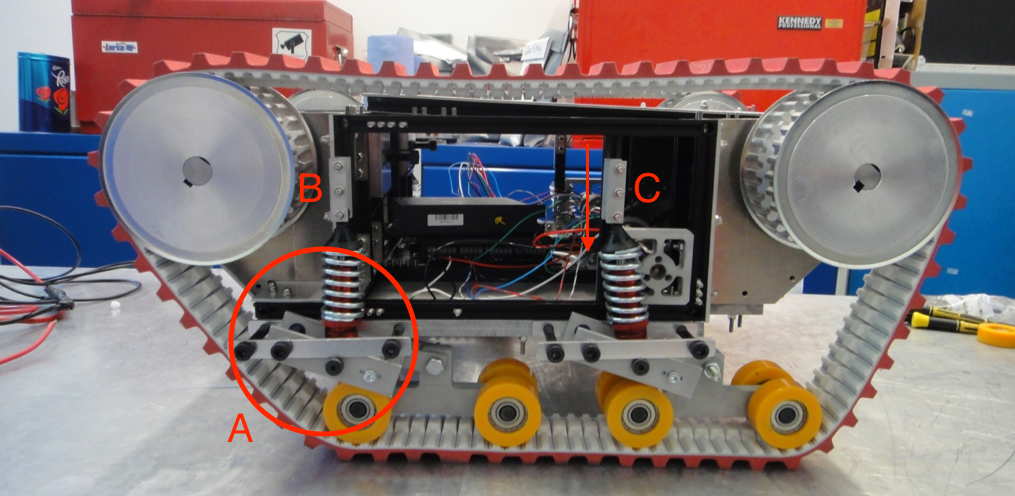
\includegraphics[width=0.6\linewidth]{Images/MaxImages/LHOrion.png}
\caption{Left Hand Suspension from 2014/2015 Technical Report}
\label{fig:LHOrion}
\end{figure}
The design and mounting of the outer mounting plates also cause problems. As can be seen in Figure \ref{fig:LHOrion}  there is no spacer between the inner and outer mounting plates. When the mounting bolts (A on the image) are tightened they bend the outer mounting plates inwards towards the robot. This bending increases frictions as the swing-arm pivot and traps the swing-arm preventing it from rotating.\par

The mounting blocks for the top of the coil spring are also flawed. The are bolts holding them to the MakerBeam chassis elements are perpendicular to the force of suspension compression, there is not restraint in the axis of compression. This means that under high compression events, e.g. a drop from 350mm, the mounting block slips upwards, further any suspension travel to zero. It was found that moving the mounting blocks downwards, illustrated as C in Figure \ref{fig:LHOrion}  rotated the swing-arm so that the spring mounting bolt would not foul the outer mounting plate under compression. This set-up is not ideal however, as it raises the ride height and centre-of-gravity significantly.\par

The suspension assemblies are mounted to the baseplate of the robot with three M6 bolts. When the robot is dropped from the test height of 350mm all of the impact force will be transferred into the baseplate via the four sets of three bolts as none of the energy will be absorbed by the suspension as it cannot compress due to design limitations. The thread depth is 20mm and the length of unsupported bolt is 41mm. Repeated loading of these bolts is likely to damage the shallow threads in the aluminium baseplate, rendering it unusable. \par

Due to the design of the suspension the outer mounting plates and bolts sit outside the outer line of the tracks, shown in Figure \ref{fig:OrionFront}. This makes the robot wider than it could otherwise be as well leaving these delicate components vulnerable in the event of a crash or roll-over. \par

\begin{figure}[h]
\centering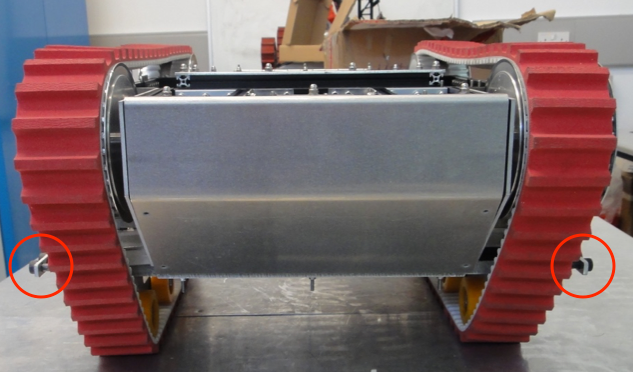
\includegraphics[width=0.6\linewidth]{Images/MaxImages/OrionFront.png}
\caption{Exposed Suspension Mounting Hardware}
\label{fig:OrionFront}
\end{figure}

The design has 16 pivoting joints in total, all of which are wear surfaces and will require lubrication and maintenance. This is not ideal for an urban search and rescue robot which will operate in harsh environments where particulate matter may contaminate bearing surfaces. The bearings used were all small (4mm I.D, 5mm width) sealed cartridge ball-bearings, replacing these in a field situation would be a tedious task. Furthermore, as the bearings were small the bearing surface was also small. This meant that each bearing was subjected to a high load during testing and operation. This loading would likely cause premature wear and resistance of the suspension linkage, compromising performance.

Overall the design is complex and difficult the assemble. There are nine parts for each suspension assembly that must be aligned correctly and held in position to be threaded in to place. The mounting bolts must also be not be over-tightened to avoid bending the outer mounting plates and locking the suspension, further complicating in-field repairs. 

The coil spring design also lacks adjustability. The springs do have adjustable reload, however there is no mechanism for adjusting the spring rate or ground clearance of the vehicle without disassembling the whole suspension system, which is a time consuming and complex task. This means that the suspension cannot be levelled if there is uneven weight distribution of the robot.


A positive aspect of this coil-spring design is relatively low un-sprung mass and the damping built into the coil spring units. The damping was beneficial because it stops the suspension from oscillating between compression and extension following an impact, returning the suspension to the neutral position more quickly.

The suspension design could have been modified to improve the performance, for example mounting spacers to prevent the mounting plates from bending inwards and fouling the mounting bolts. The lack of sag could be addressed by moving the upper coil spring mounting points lower or replacing the coil springs for longer units, however this would further increase the height of the centre of gravity, which is not desirable. Overall, due to the limitations of the design and lack of robustness, a new suspension design was most appropriate, as the what was learnt from the shortcoming of the coil spring design could be used to create higher performance suspension more suited to the needs of the robot.

\subsubsection{Review of Possible Alternative Suspension Designs}
Several alternative suspension designs were considered to replace the current coil spring design. The alternatives were considered on function, manufacturability and weight. All alternatives would have to improve on the current design to be a realistic option.\par

The first option to be considered was removing the suspension entirely and fixing the idlers directly to the base plate of the robot. Such a design would the the simplest, lightest and most robust as there are no moving parts nor extra mechanisms needed. However, as explained in the section titled “Why Have Suspension” there are many benefits to having a form of suspension and it was thought that removing it would limit the capabilities of the robot. \par

A second option considered was modifying the current suspension to rectify some of the problems it has with components fouling each other and bending when tightened properly. This would have a lower design and manufacturing time than re-designing from scratch. It was decided however, that the time savings were not worth the significant drawback in the design, namely the complexity and fragility.\par

Traditional suspension designs for tracked vehicles were then reviewed and considered. A type of suspension that has been used for tracked vehicles is Christie suspension. It is comprised of a coil spring mounted horizontally which is actuated by a bell-crank \cite{Mastinu11}. Christie suspension provides a large range of motion but reduced the internal volume of the chassis \cite{Zaloga15}. To contain all the internal components of the robot it is not feasible to reduce the internal volume, so this design was disregarded. 
\par

The most widely used type is torsion bar suspension \cite{Mastinu11}. Torsion bar suspension uses a bar mounted to a swing arm to provide a spring action in torsion (Figure \ref{fig:torsionbar}). One end of the torsion bar is fixed to a swing-arm on which a road wheel is mounted and the other end is fixed to the hull of the vehicle \cite{Mastinu11}. \par
\begin{figure}[h]
\centering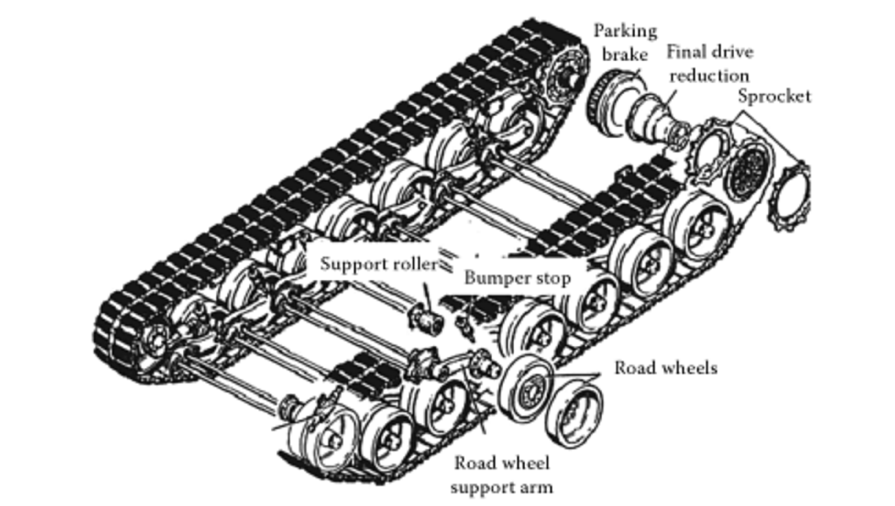
\includegraphics[width=0.6\linewidth]{Images/MaxImages/torsionbarsus.png}
\caption{Torsion Bar Suspension \cite{Mastinu11}}
\label{fig:torsionbar}
\end{figure}
The torsion bar design has been widely adopted because of its simplicity lightweight associated with this. Torsion bar suspension also stores more energy for the same weight than other systems do, further reducing weight \citet{Hohl85}. Torsion bars can be mounted inside the vehicle to project from damage or underneath the vehicle to increase interior volume, the second option would be suitable for the robot as maximum interior volume is needed to house the electronic components and the suspension should not protrude past the outside line of the tracks. Whilst the bars may be vulnerable to damage sitting outside the chassis the components are simple to replace \cite{Hohl85}. 

The spring rate of torsion bars can be changed by changing the the diameter of the bar or the length so it could be possible to include an adjustment mechanism in a design to change the spring rate and therefore the ride-height, allowing the robot to be levelled. Such adjustability would allow the pitch of the chassis to be changed depending on terrain conditions, improving tractive performance \cite{Wong88}. The shorter a torsion bar is the, stiffer and therefore the higher the spring rate.

\[ k = \frac{ \pi\times d^4 \times G}{32L} \]
\[k = spring\:rate\:(N/m), d = diameter\:(m), G = Young's\:modulus\:(N/m^2), L = length\:(m)\]

There are some disadvantages, however. Torsion bars do not self-damp \cite{Hohl85}, so either dampers will need to be included in the design or not used. Whilst not using dampers for a fast-moving tracked vehicle would be unfeasible the robot travel at a maximum speed of 0.5m/s and will weigh less than 25kg. Firstly, it is likely that the robot will be travelling too slowly for any large oscillations to be induced and secondly there will be a degree of coulomb (sliding friction) damping \cite{Persson00} in the suspension system, especially the dynamic tensioners which will feature steel rod sliding through an aluminium block in the direction opposite to suspension compression or extension. Secondly, the spring rate of torsion bars is linear, not progressive as coil springs are \cite{Hohl85}. For larger vehicles progressive spring rates are preferable, however it is an acceptable compromise in return for a robust and simple suspension system.

Overall it was deemed that the advantages of torsion bar suspension, namely; simplicity, light weight, robustness, the potential for adjustability, no reduction in internal volume and good packaging outweighed the disadvantages of no inherent damping and linear spring rate. 


\subsubsection{Design of Orion's Torsion Bar Suspension}
To summarise, torsion bar suspension was chosen for the following reasons in Table 1. These reasons formed the basis of the suspension requirements. The suspension design must fulfil these requirements.
\begin{table}[h]
\centering
\begin{tabular}{l}
\hline
Good performance\\
No internal volume lost\\
Adjustable\\
Robust\\
Simple\\
Easy to manufacture\\
Low external profile\\
\hline
\end{tabular}
\caption{Reasons for Torsion Bar Suspension}
\end{table}

When designing the torsion bar suspension, it was a priority to keep all parts as simple as possible. Reducing complexity makes the design and manufacturing phases shorter, improves the reliability of a design and takes in-service maintenance and repair simpler. The current suspension was analysed to determine which components could be reused. It was decided to reuse the idlers from the previous design and well at retain the same swing arm length of 80mm \par

Suspension design was started by calculating the dimensions of the components critical to the function of the suspension. Firstly, the amount of suspension travel needed to be decided. The previous design had a total spring travel of 25mm, allowing a maximum compression of 12mm, as spring are not recommended to compress more than half of their travel. There is no maximum travel of torsion bar suspension. As long as the shear stress in the torsion bar does not exceed the shear modulus of the material the suspension will continue to function. It was decided that a reasonable twist angle under maximum compression (dropping the robot from 350mm) was 20° (0.35rad) from the starting position to the horizontal. This gave approximately 27mm, 2.25 times the travel of Orion. The suspension was able to rotate a further 5.7° (0.1rad) past the horizontal before bottoming out. This zone is not intended for normal operation and is there to prevent the suspension from running out of travel and contracting the shell.\par

\begin{equation}
T= sin(\theta) \times L
\end{equation}

\[T = sin(0.35) \times 80 = 27mm\]


Figure \ref{fig:SwingDiag} shows the path of the swing-arm under compression. The swing-arm starts at “S”, the neutral position and can be compressed normally to anywhere in the zone marked by the green dotted line. The swing angle (Θ$_1$ ) in this zone is 20° (0.35rad). The zone marked by the red dotted line is the extra travel which is not meant to be used but guards against the swing-arm from contacting the chassis during compression. The swing angle (Θ$_2$ ) in this zone is 5.7° (0.1rad).

\begin{figure}[h]
\centering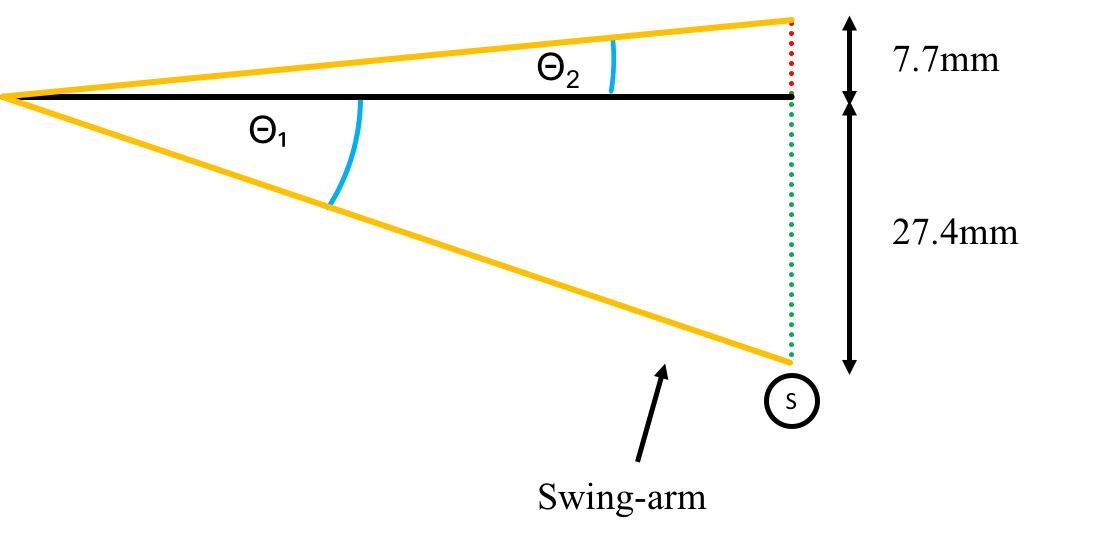
\includegraphics[width=0.6\linewidth]{Images/MaxImages/Swing_Diag.png}
\caption{Suspension Compression Path}
\label{fig:SwingDiag}
\end{figure}

Another consideration of travel is ground clearance and centre of gravity. The centre of gravity of Orion 2014 was relatively high \textcolor{red}{(prove this)}and it was felt that the robot did not need as much clearance.\par SAY SOMETHING

Having determined the length of the swing-arm and the swing angle for the travel needed when dropped from 350mm the force of this drop was calculated given a robot weight of 25kg. The force was calculated to be 738N (3 S.F) per corner, giving a torque on the torsion bar of 62.7N (3 S.F).\par
\begin{equation}
 F = \frac{m \times g \times h}{stopping\:distance} = \frac{25 \times 9.81 \times 0.35}{0.0274} = 3132.775N
\end{equation}

\[\frac{3132.775}{4} = 783.189N \approx 783N\]

\begin{equation}
T = F \times d\ = 783.189 \times 0.08 = 62.655Nm
\end{equation}

The polar moment of inertia of a torsion bar of a given cross-section was calculated as well as the length of bar needed to allow a 20°m swing angle for three materials of bar (magnesium, aluminium and steel). The sections considered were cylindrical and rectangular The dimensions of the torsion bar and blade were modified in an Excel model to give a suitable length of bar that would allow good adjustability. 

\begin{equation}
Circular\:section: J = \frac{\pi(d^4)}{32}
\end{equation}

\[J = \frac{\pi(0.006)^4}{32} = 12.72\times 10^{-11}m^4\]

\begin{equation}
Rectangular\: section: J = \frac{bh}{12}(b^2 + h^2)
\end{equation}


\[J = \frac{0.00635\times0.002}{12}(0.00635^2 + 0.002^2) = 4.69\times10^{-11}m^4\]

The minimum maximum length of torsion bar needed to absorb a fall from 350mm if the robot were to weight 25kg was calculated. The overall width of the robot was to remain the same, therefore the maximum length of the torsion bars was 119mm, leaving a 10mm gap between the left- and right-hand bars. Subtracting material thicknesses gave an adjustable range of 99mm. Torsion bar lengths were calculated for all materials. The results showed that the most suitable material for a torsion bar was 6mm diameter aluminium, needing a length of 49.0mm to absorb the fall; a steel torsion blade (6.35mm by 2mm) needed to be 52.4mm. Both lengths give a wide range of adjustability in the 99mm maximum length, allowing the suspension to be softened and lowered or stiffened and raised as needed.\par

\begin{equation}
Length = \frac{\theta(J \times G)}{T}
\end{equation}

\[\theta = Twist\:angle\:(radians), J = polar\:moment\:of\:inertia (m^4),\]
\[G = Young's\:modulus (N/m^2), T = Torque (Nm)\]

\[Aluminium\:bar: L = \frac{0.35(12.72\times 10^{-11} \times 45 \times 10^{-9})}{62.64}\]
\[L = 0.0490m = 49.0mm\]

\[Steel\:blade: L = \frac{0.35(4.69\times10^{-11} \times 200 \times 10^{9})}{62.64}\]
\[L = 0.0524m = 52.4mm\]
The steel blade was more suitable because of the higher sheer modulus of steel (79GPa) against aluminium (25.5GPa) (Crandall78), which is critical as the torsion bars will experience significant shear force. Furthermore, from a manufacturability standpoint it would be easier to fix a flat blade to other component than a cylindrical bar. Using a steel torsion bar was investigated but found to be unfeasible due to the small diameter required for a good range of adjustability.

Spring rate was calculated to determine the spring rate of needed for the dynamic tensioning system. The spring rate of all materials and their respective lengths was the same as they all had to absorb the energy from the drop, therefore the spring rate was calculated using the data for the 6mm aluminium bar, as is simplified calculations.

\begin{equation}
Spring\:rate = \frac{\pi \times d^4 \times G}{34L}
\end{equation}

\[Spring\: rate = \frac{\pi \times 0.006^2 \times 45\times10^{9}}{34\times 0.00490} = 179.0 N/m\]

A rail system with a movable anchor point for the torsion blade was designed to allow the effective length to be varied to adjust spring rate and therefore travel and ground clearance. The rail system would be made from MakerBeam. There were concerns that the “wings” of the MakerBeam would not withstand the tensile and compressive forces subjected to the suspension during compression. A simulation was run on on the MakerBeam rails (Figure \ref{fig:SuspensionSim3}), subjecting one side to tensile stress and the other to compressive stress, as would happen when the suspension is compressed and the blade under torsion, which is then transferred to the baseplate via the MakerBeam. The tensile and compressive loads simulated were 10000N, significantly higher than the robot would see under normal operation. The MakerBeam plastically deformed by approximately 0.01mm and is subjected to stress of \textcolor{red}{INSERT INFO HERE}.

\begin{figure}[h]
\centering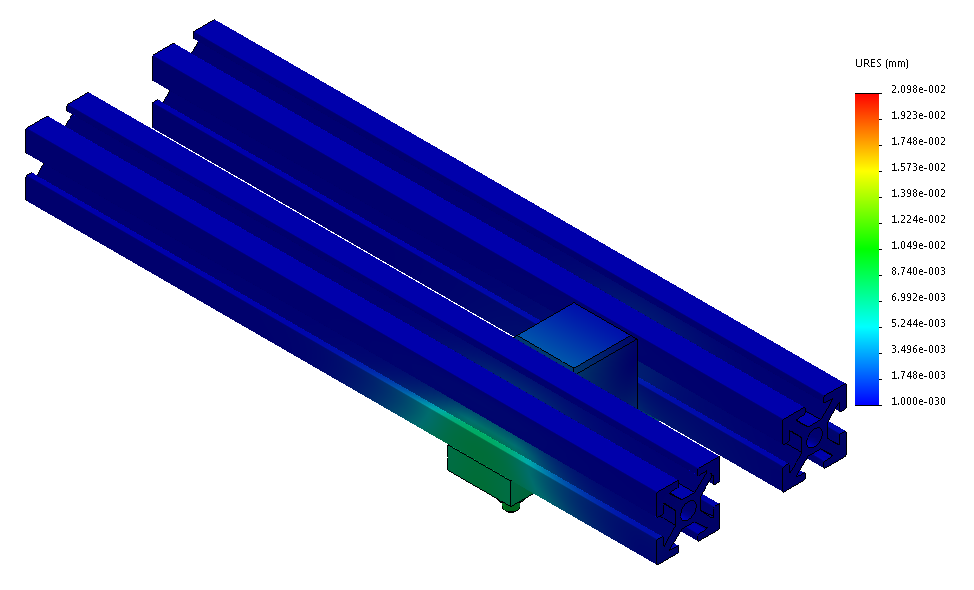
\includegraphics[width=0.6\linewidth]{Images/MaxImages/Suspension_beam_sim_3.png}
\caption{MakerBeam Rail Deformation}
\label{fig:SuspensionSim3}
\end{figure}
The machine screws fixing the tuning block to the MakerBeam was subjected to approximately 380MPa under the applied loads. The yield stress of an M2.5 scews is 1300MPa (Viewmold16), therefore the stress that will be exerted on the screws during normal operation will not exceed the yield stress of the fixings. This is shown in Figure \ref{fig:SuspensionSim1}.
\begin{figure}[h]
\centering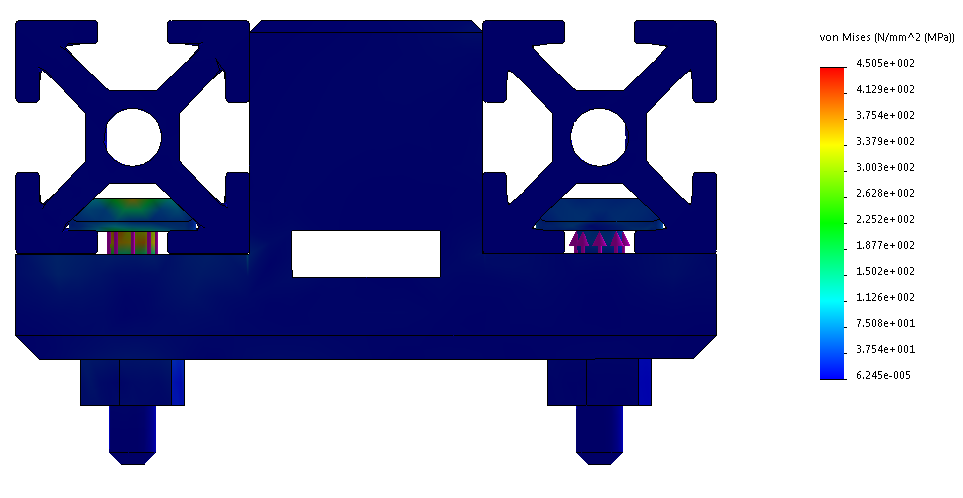
\includegraphics[width=0.6\linewidth]{Images/MaxImages/Suspension_beam_sim_1.png}
\caption{Stress on MakerBeam Fixings}
\label{fig:SuspensionSim1}
\end{figure}
Where possible components were designed to be as close to stock material sizes as possible to reduce manufacturing time. An example of this are the swing-arms. The first design used a heavily contoured part that would have to be CNC machined. The set-up of this process would have been time consuming due to the intricacy of the design. The swing-arm was redesigned to make manufactured from a stock U-section. The aluminium extrusion would be stiffer than previous design and simpler to manufacture. The section could be cut to length and the appropriate holes drilled with no significant machining required. 

INSERT IMAGES OF BOTH SAs

2014/2015’s Orion used 8 small sealed ball-bearing cartridges (4mm I.D, 5mm width) through which all the impact force from the terrain was transferred into the chassis. To improve on this polymer plain bearings were used, again 8, however width was 10mm, providing double the bearing surface. A second advantage of was that the polymer will not corrode, unlike the previous steel bearings. The robot could operate in harsh environmental conditions making corrosion resistance a consideration.

The torsion bar suspension set-up fitted to Cyclone was designed using the lessons learnt form Orion as guidance. The problems highlighted in the critical analysis of the suspension are all problems which could disable the robot in the field and the new design sought to address theses. The torsion bar suspension, while undamped, did address the issues of the coil spring design and would provide a more robust system that is also simpler. Table \ref{fig:SusComp} compares the suspension systems of Orion and Cyclone.

\begin{table}[h]
\centering
\begin{tabular}{l l l}
\hline
\textbf{} & \textbf{Orion 2014} & \textbf{Orion 2016}\\
\hline
Travel & 12mm & 27mm\\
Ground Clearance & 100mm & 93mm \\
Adjustability & Fixed travel \& ground clearance&  Adjustable travel \& ground clearance\\
Pivot Points & 16 & 8\\
Parts Count & 16 & 16\\
\hline
\end{tabular}
\caption{Comparison of Orion's and Cyclone's Suspension}
\label{fig:SusComp}
\end{table}

\subsubsection{Simulation of Suspension Components}

To assist the design and validation of the suspension components stress simulations were carried out. The service conditions of the components were known and were used to form the basis of the simulations. If the components exceeded the materials yield strength or did not perform satisfactorily the design, dimensions or materials were changed.

\paragraph{Blade Adapter}

Figure \ref{fig:BladeAdapterSim} is a simulation applying 783N (the calculated force on one suspension assembly when dropped from 350mm) in the Y-axis to the smaller diameter section of the blade adapter. This simulated what would happen if the torsion blades were set far too short and not allowed to function as springs. This would transfer all of drop force into the blade adapter. From the image it is clear that the maximum stress (134.9MPa) is lower than the yield stresses of 6063-T6 aluminium (215MPa) (Davis93) and silver steel (640MPa) (Smith94). The decision was made to manufacture the component from silver steel as it allows a greater factor of safety as well as a better bearing surface when compared to aluminium. Furthermore, the average stress on the blade adapter is 50MPa, 5x lower than the yield stress of silver steel.

\begin{figure}[h]
\centering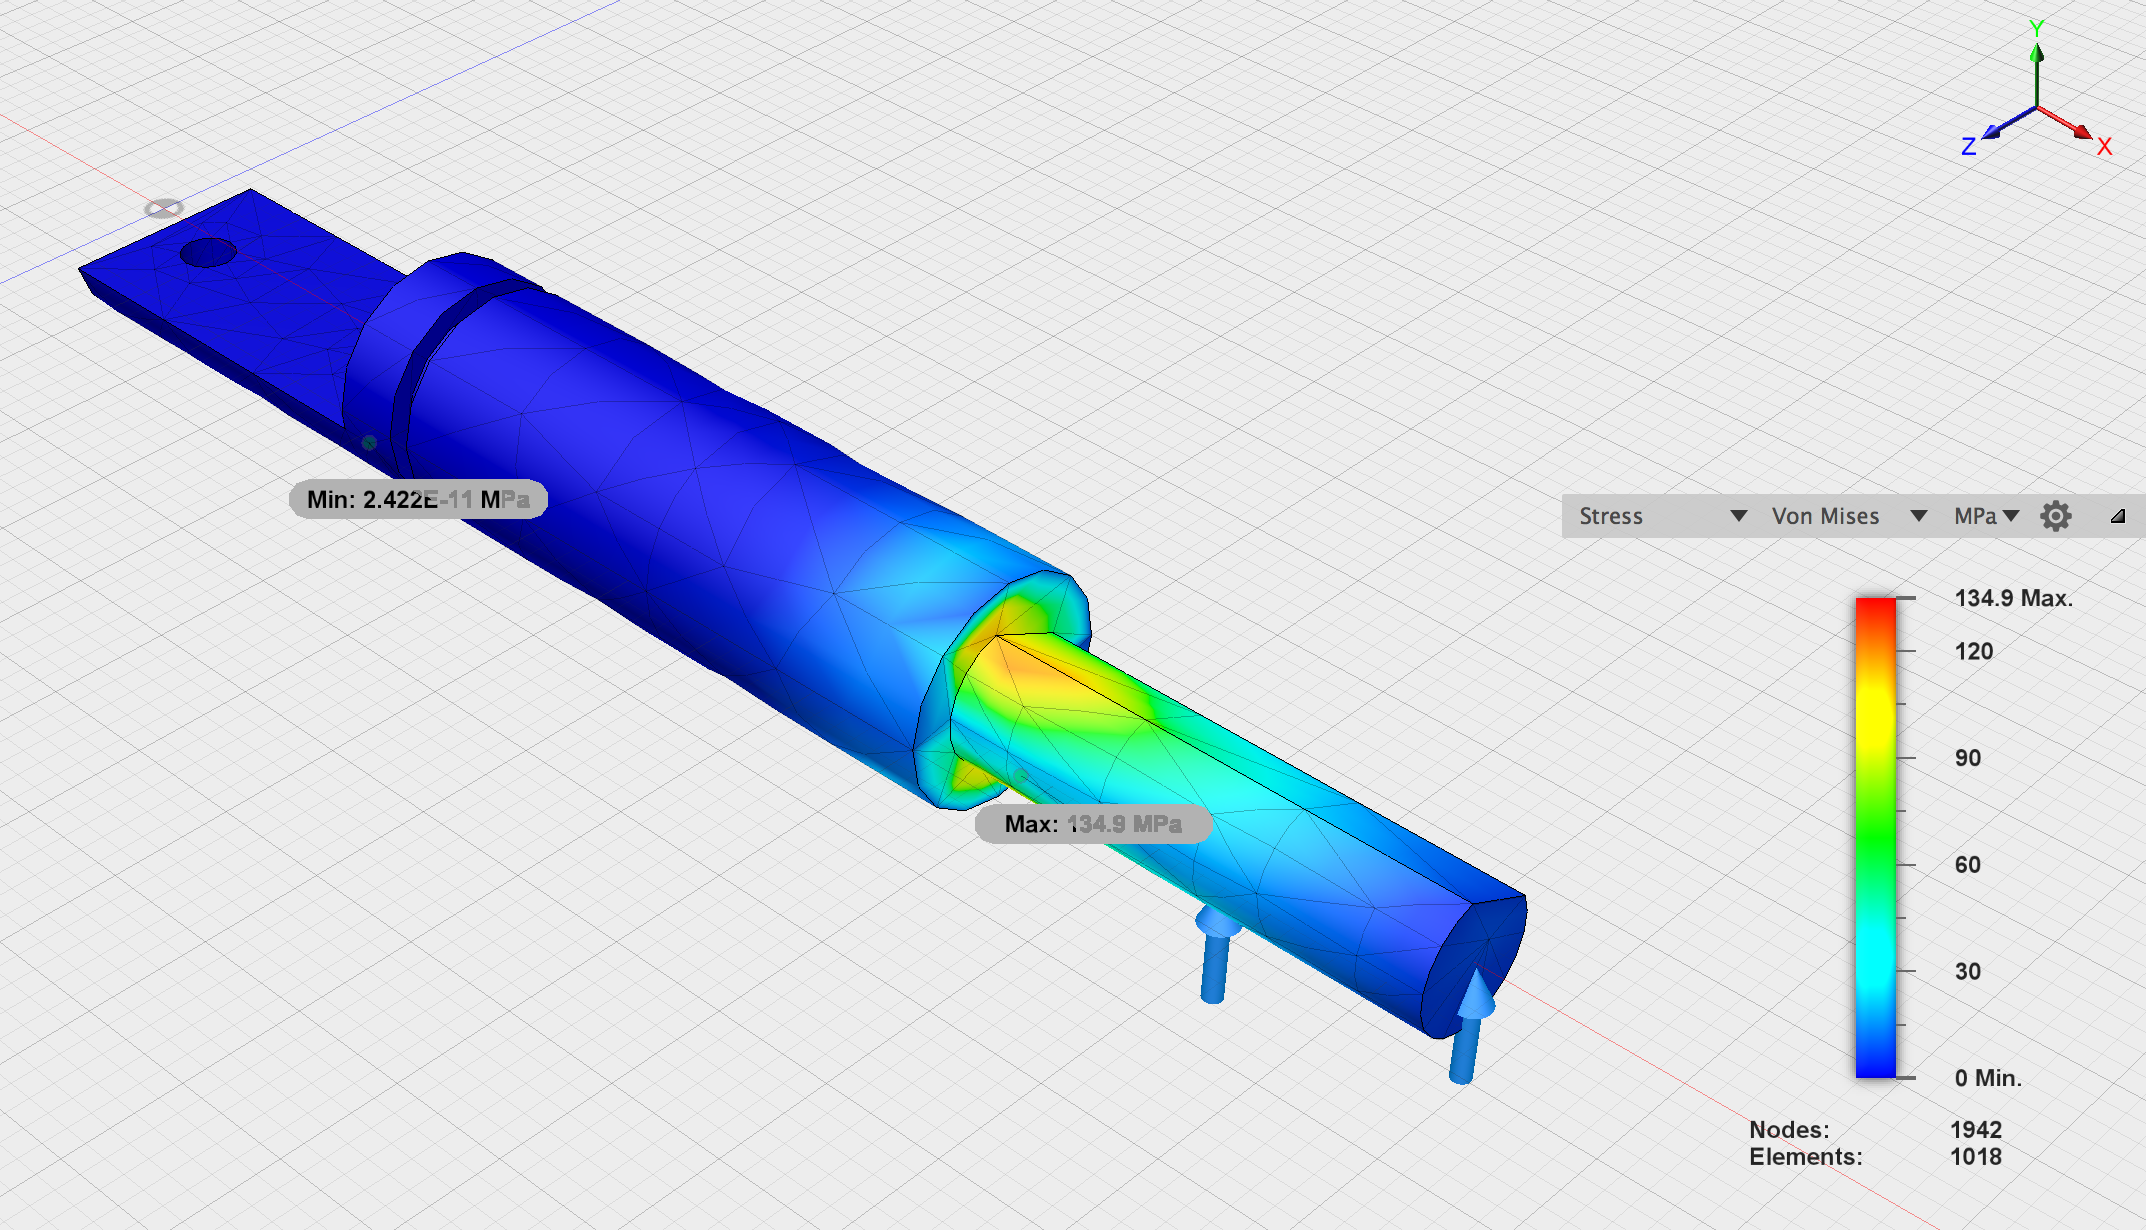
\includegraphics[width=0.6\linewidth]{Images/MaxImages/BladeAdapterSim.png}
\caption{Simulation of the Blade Adapter}
\label{fig:BladeAdapterSim}
\end{figure}

\paragraph{Torsion Blade and Blade Adapter}

Simulations investigating the shear stress on the torsion blade and  blade adapter were also run. When a torque of 62.64 Nm (the torque when dropped from 350mm) is applied to the blade adapter the maximum shear stress on blade adapter is 4042MPa (4.042GPa), the minimum stress is -7237MPa (-7.237GPa), which can be treated as 7237MPa (7.237GPa). The shear modulus of steel is 79GPa (Crandall78), giving a factor of safety of over 10x. The average shear stress on the blade adapter is around 80MPa (0.08GPa) and around 1800MPa (1.8GPa) on the torsion blade, as seen in Figure \ref{fig:TorsionBladeandAdapter}, and will therefore have an even greater factor of safety. This means that during normal operation the shear stresses exerted on the blade adapter and torsion blade will not cause the components to plastically deform.

\begin{figure}[h]
\centering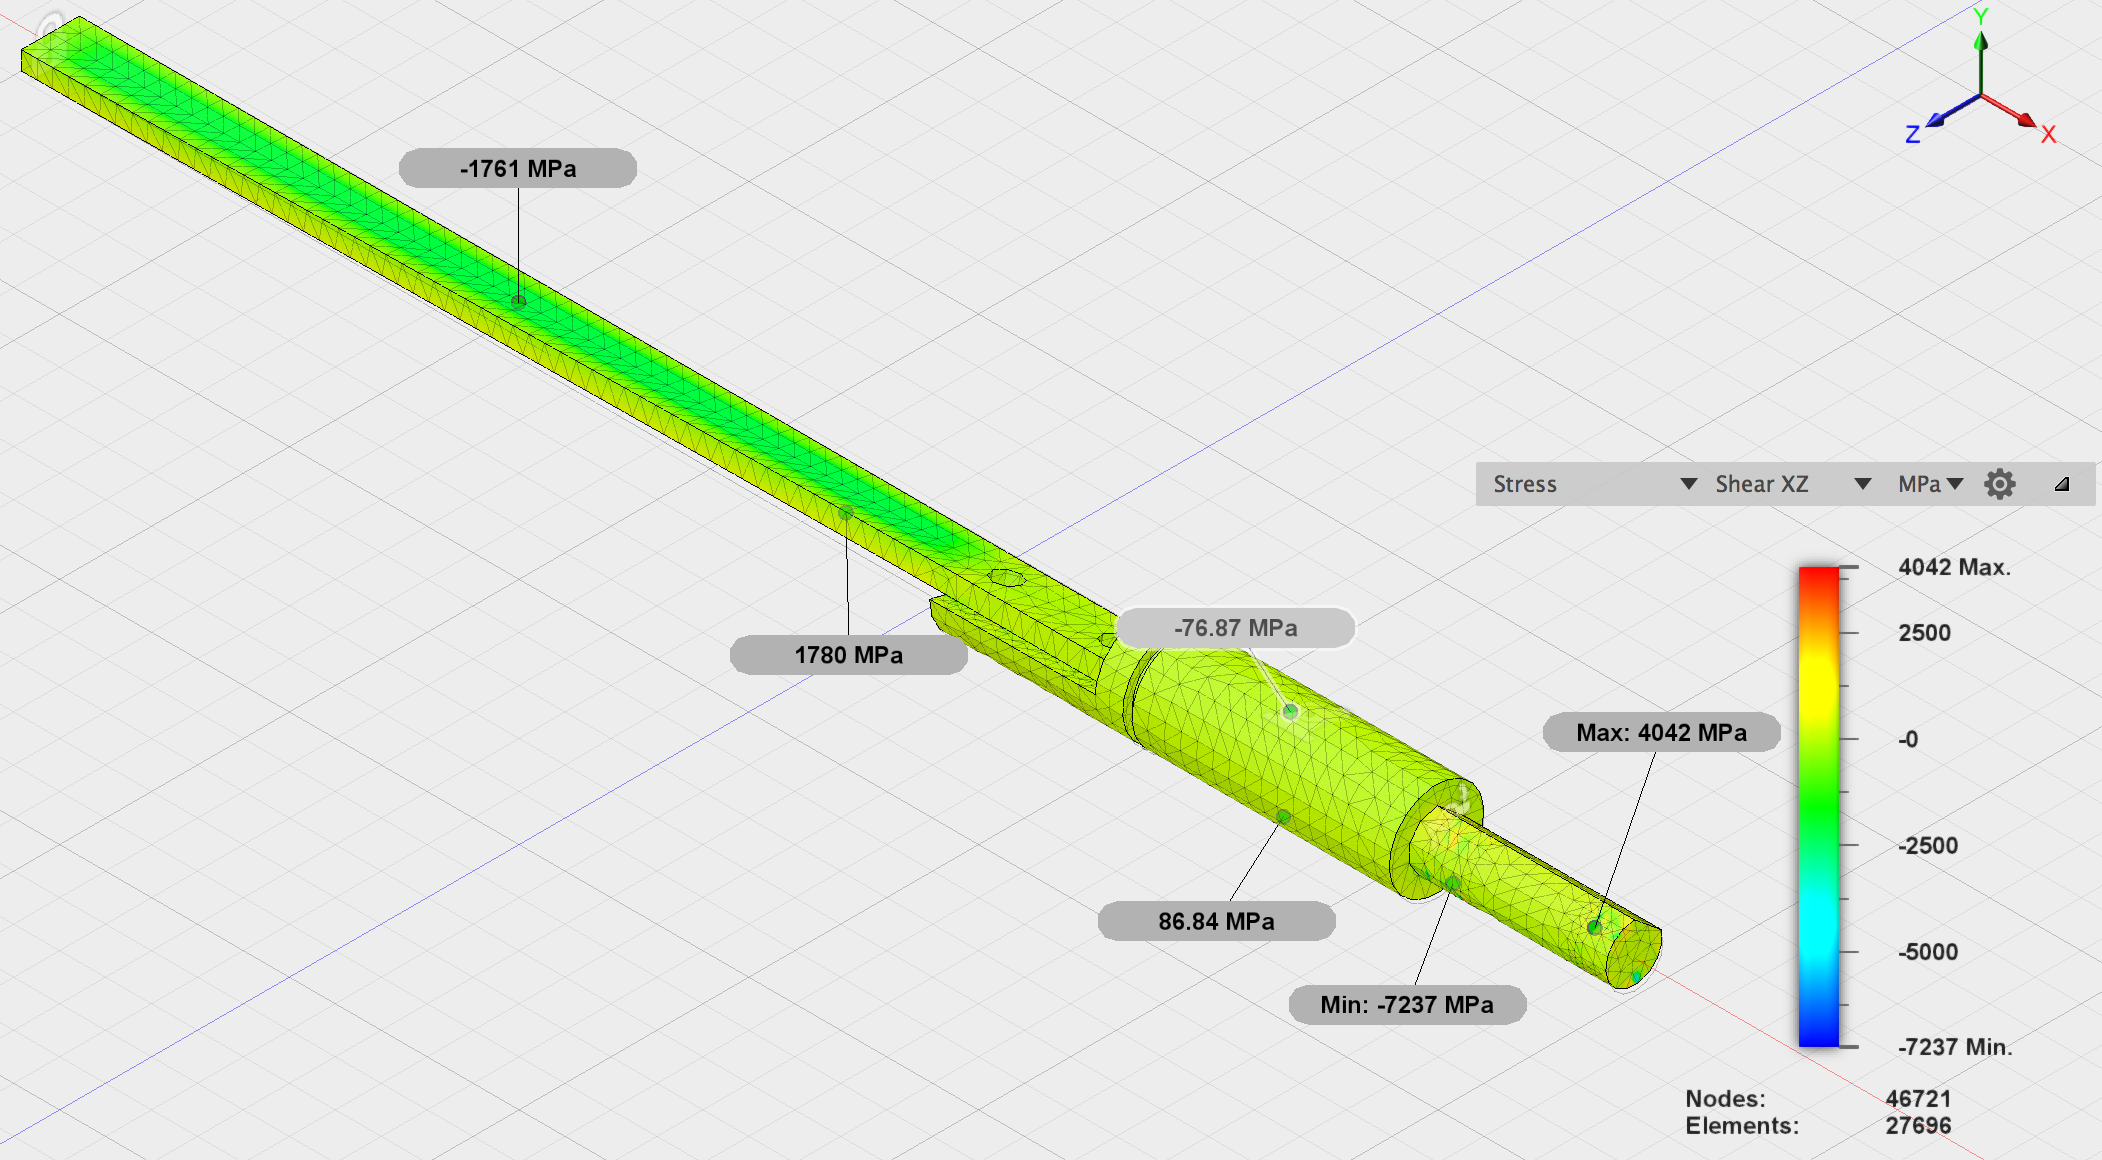
\includegraphics[width=0.6\linewidth]{Images/MaxImages/TorsionBladeandAdapter.png}
\caption{Simulation of the Torsion Blade and Blade Adapter}
\label{fig:TorsionBladeandAdapter}
\end{figure}